\documentclass[dvipdfmx,autodetect-engine]{jsarticle}
\usepackage[dvipdfm]{graphicx}
\usepackage{ascmac}
\usepackage{fancybox}
\usepackage{listings}
\usepackage{plistings}
\usepackage{itembkbx}
\usepackage{amsmath}
\usepackage{svg}
\usepackage{url}
\usepackage{graphics}
\usepackage{listings,jvlisting}
\usepackage{here}

\textheight=23cm
\renewcommand{\figurename}{図}
\renewcommand{\tablename}{表}
\newenvironment{code}
{\vspace{0.5zw}\VerbatimEnvironment  
\begin{screen} 
\baselineskip=1.0\normalbaselineskip
 \begin{Verbatim}}
{\end{Verbatim}
\baselineskip=\normalbaselineskip
 \end{screen}\vspace{0.5zw}} 

 \title{プロセスログの調査によるランサムウェアの動的解析} 
 \author{山下恭平、塚本覇虎、奥若菜}
 \date{2022年7月30日}
 \begin{document} 
 \maketitle

\section{実験の背景と目的}
2022年3月に独立行政法人情報処理推進機構(通称IPA)から発表された、今年注意を要するサイバー空間における「情報セキュリティ10大脅威2022」
では、法人が注意を要するとされている脅威として「ランサムウェア」が1位に挙げられている。ランサムウェアとは、感染させた端末内のデータを暗号化などによって、利用できない状態にした上で、そのデータを利用できる状態に戻すことと引き換えに身代金(金銭)を要求するマルウェアの名称である。
警察庁により公表されている企業・団体等におけるランサムウェア被害の件数は、年々増加しており、昨年(令和3年)下半期は、一昨年(令和2年)下半期と比べて約4倍になっている。\\
このように、ランサムウェアによる被害は、近年最も脅威とされ、その数も増加している。したがって、ランサムウェアをはじめとするマルウェアに対する理解を深め、その解析手法を身につけることは、情報セキュリティを学ぶ上で大変有用であると考えた。
本実験では、仮想環境でランサムウェアを実行し、その動的解析に取り組む。具体的には、ランサムウェアの実行中に得られたログから、プロセスやファイル生成の情報を調査し、どのようにデータの暗号化を行うかを明らかにすることを目的とする。
\section{実行環境}

Virtual Box上でWindowsの仮想マシンを構築し、ランサムウェアShinoLockerを
動作させ、その時のログをProcess Monitorを用いて採取した。その一覧を表1と図1にまとめる。

\begin{table}[H]
  \centering
  \caption{用いたソフトウェアとそのバージョン}
  \begin{tabular}{|c|c|}
  \hline
  ソフトウェア名                         & バージョン          \\ \hline
  Oracle Virtual Box              & 6.1.32 r149290 \\ \hline
  Windows10 Enterprise Evaluation & 1809           \\ \hline
  Process Monitor                 & 3.89           \\ \hline
  \end{tabular}
  \end{table}

  \begin{figure}[H]
    \centering
    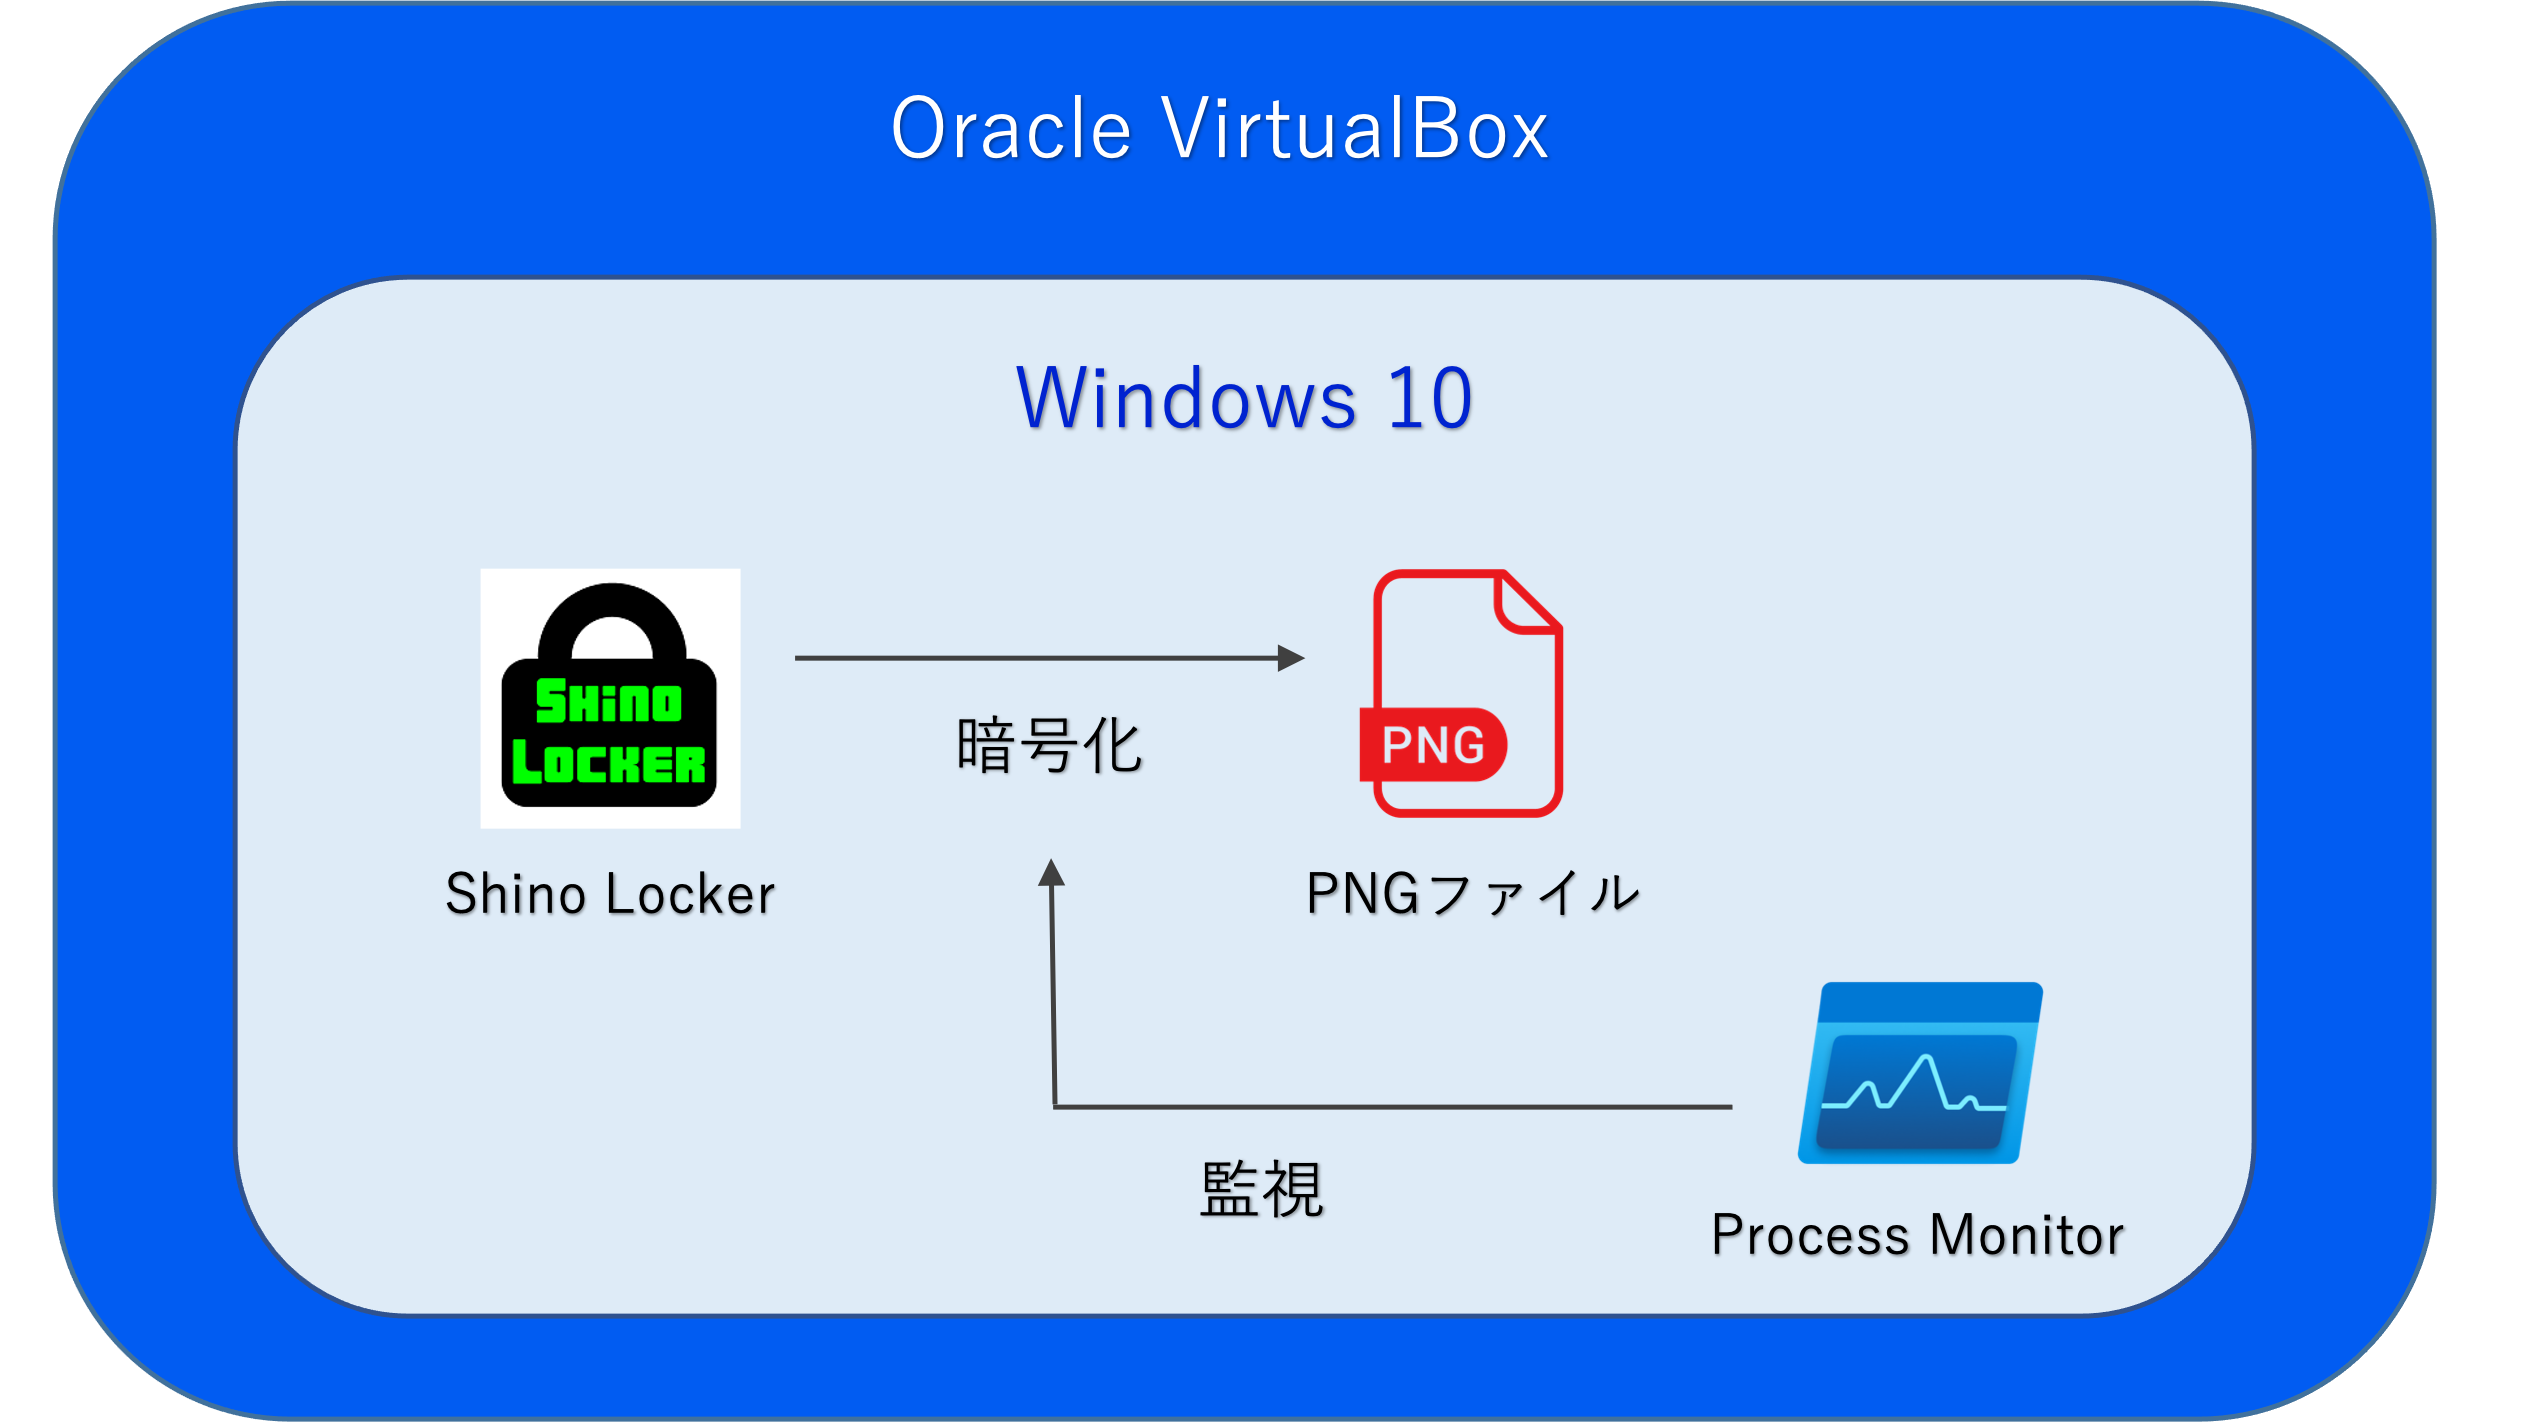
\includegraphics[scale=0.6]{pic0.png}
    \caption{実行環境図}
  \end{figure}

\section{解析対象の動作}

ShinoLockerを実際に動作させるとpngファイルが全て暗号化され、暗号化
されたファイルには「.shino」という拡張子がついていることが確認でき、さらに
アイコンが変更されていることも確認できた。また、
暗号化されたファイルを起動すると、「I9BbnQr9.exe」という実行ファイルが
呼び出され、復号するためのウィンドが表示された。その様子を図2から5へ示す。

\begin{figure}[H]
  \centering
  \begin{minipage}[b]{0.45\linewidth}
  \begin{center}
    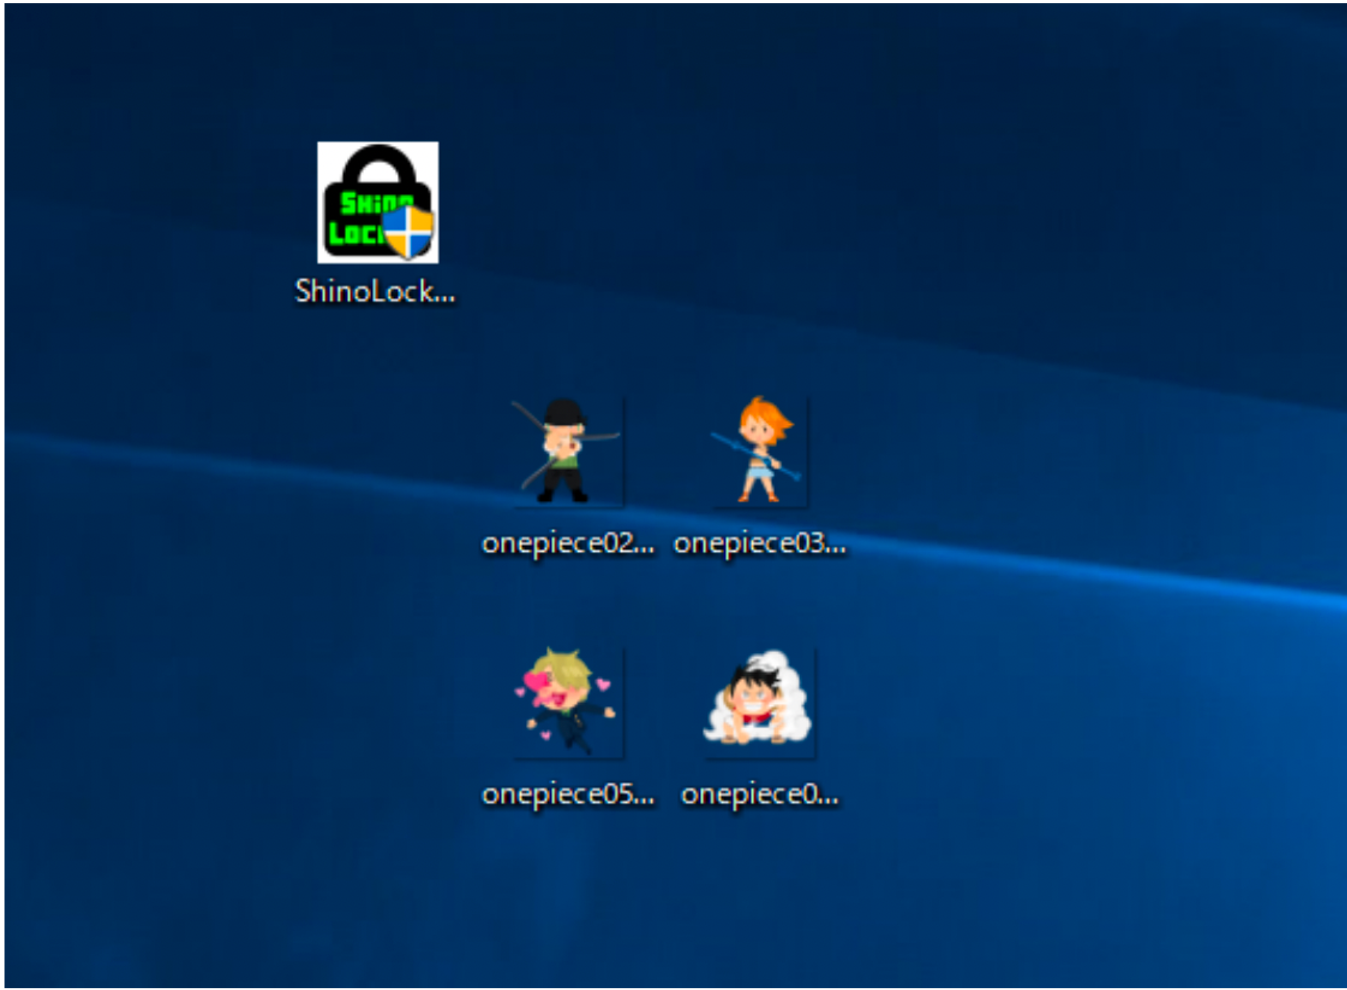
\includegraphics[keepaspectratio,scale=0.6]{pic2.png}
    \end{center}
    \caption{ShinoLocker実行前}
  \end{minipage}
  \begin{minipage}[b]{0.45\linewidth}
  \begin{center}
    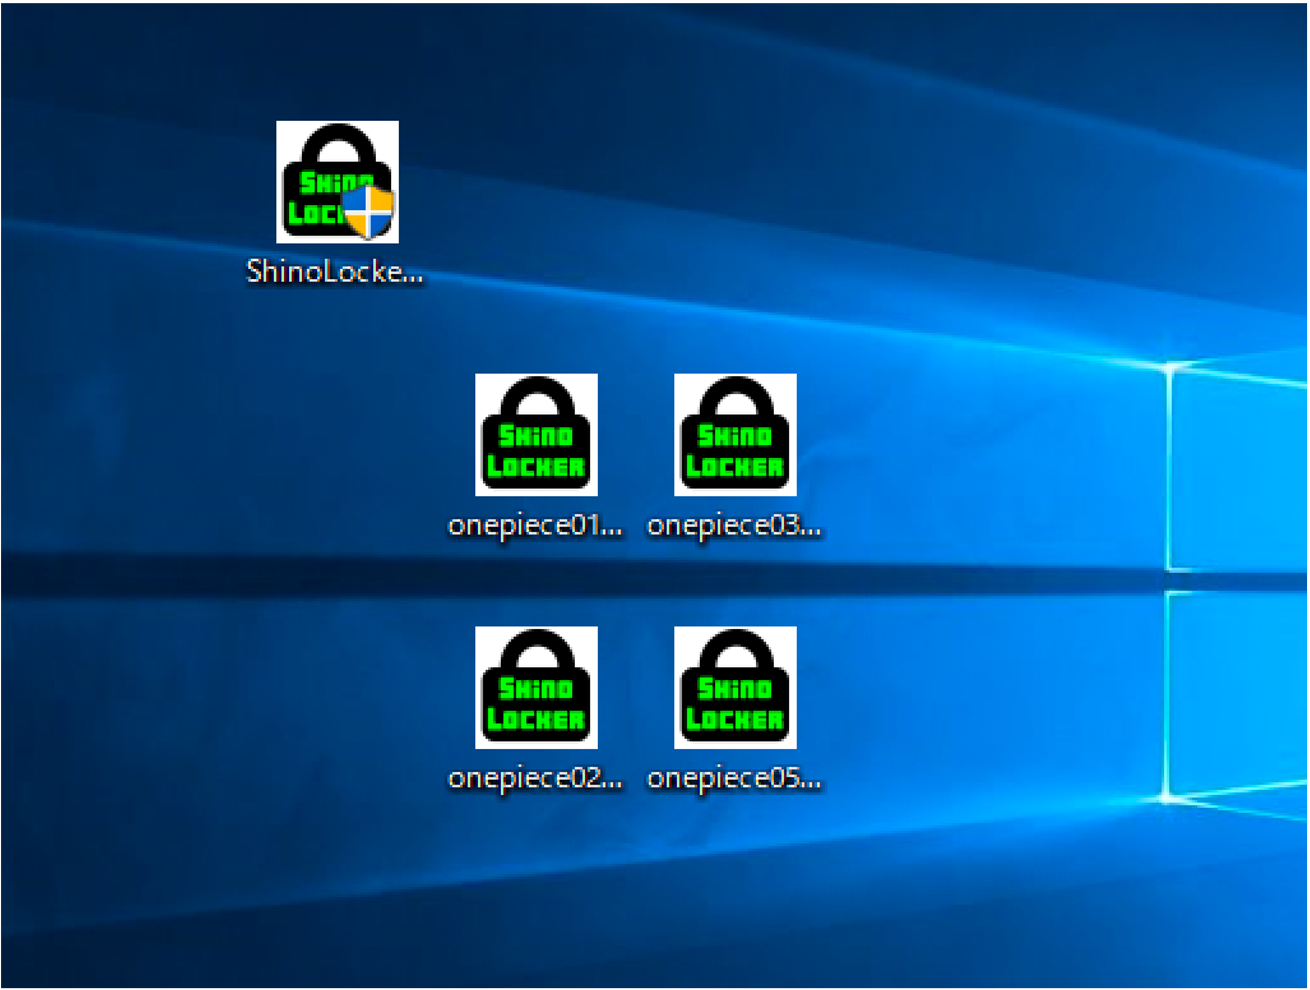
\includegraphics[keepaspectratio,scale=0.6]{pic3.png}
    \end{center}
    \caption{ShinoLocker実行後}
  \end{minipage}
\end{figure}

\begin{figure}[H]
  \centering
  \begin{minipage}[b]{0.45\linewidth}
  \begin{center}
    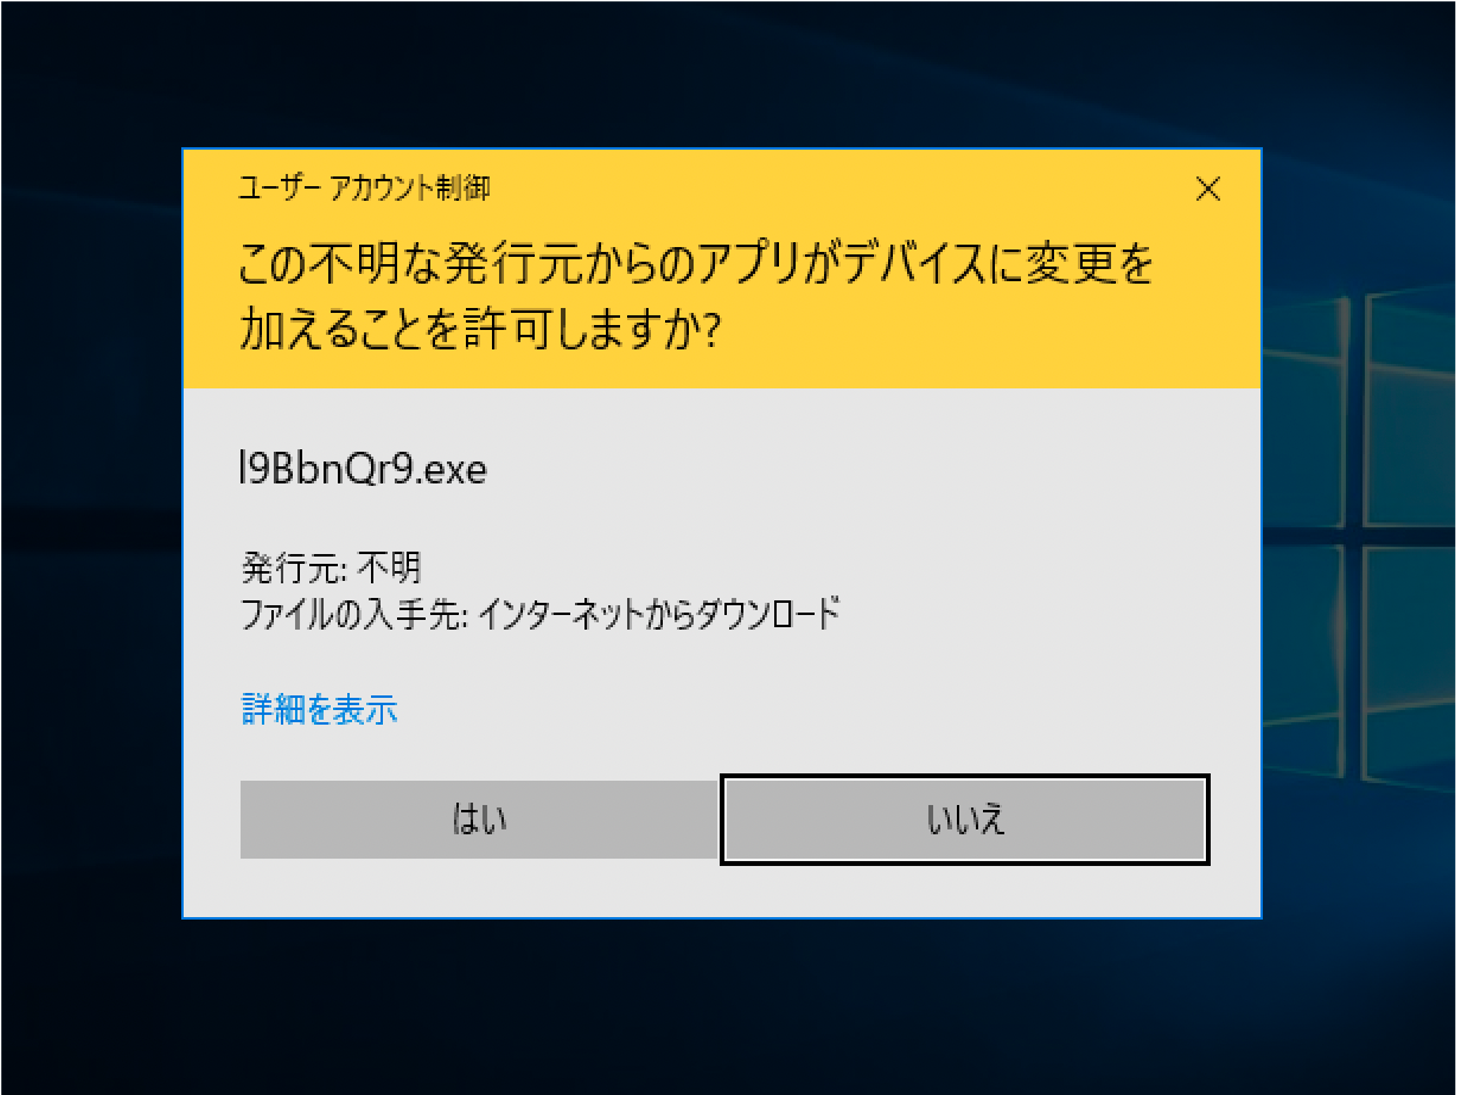
\includegraphics[keepaspectratio,scale=0.5]{pic4.png}
    \end{center}
    \caption{暗号化されたファイルを起動後の動作1}
  \end{minipage}
  \begin{minipage}[b]{0.45\linewidth}
  \begin{center}
    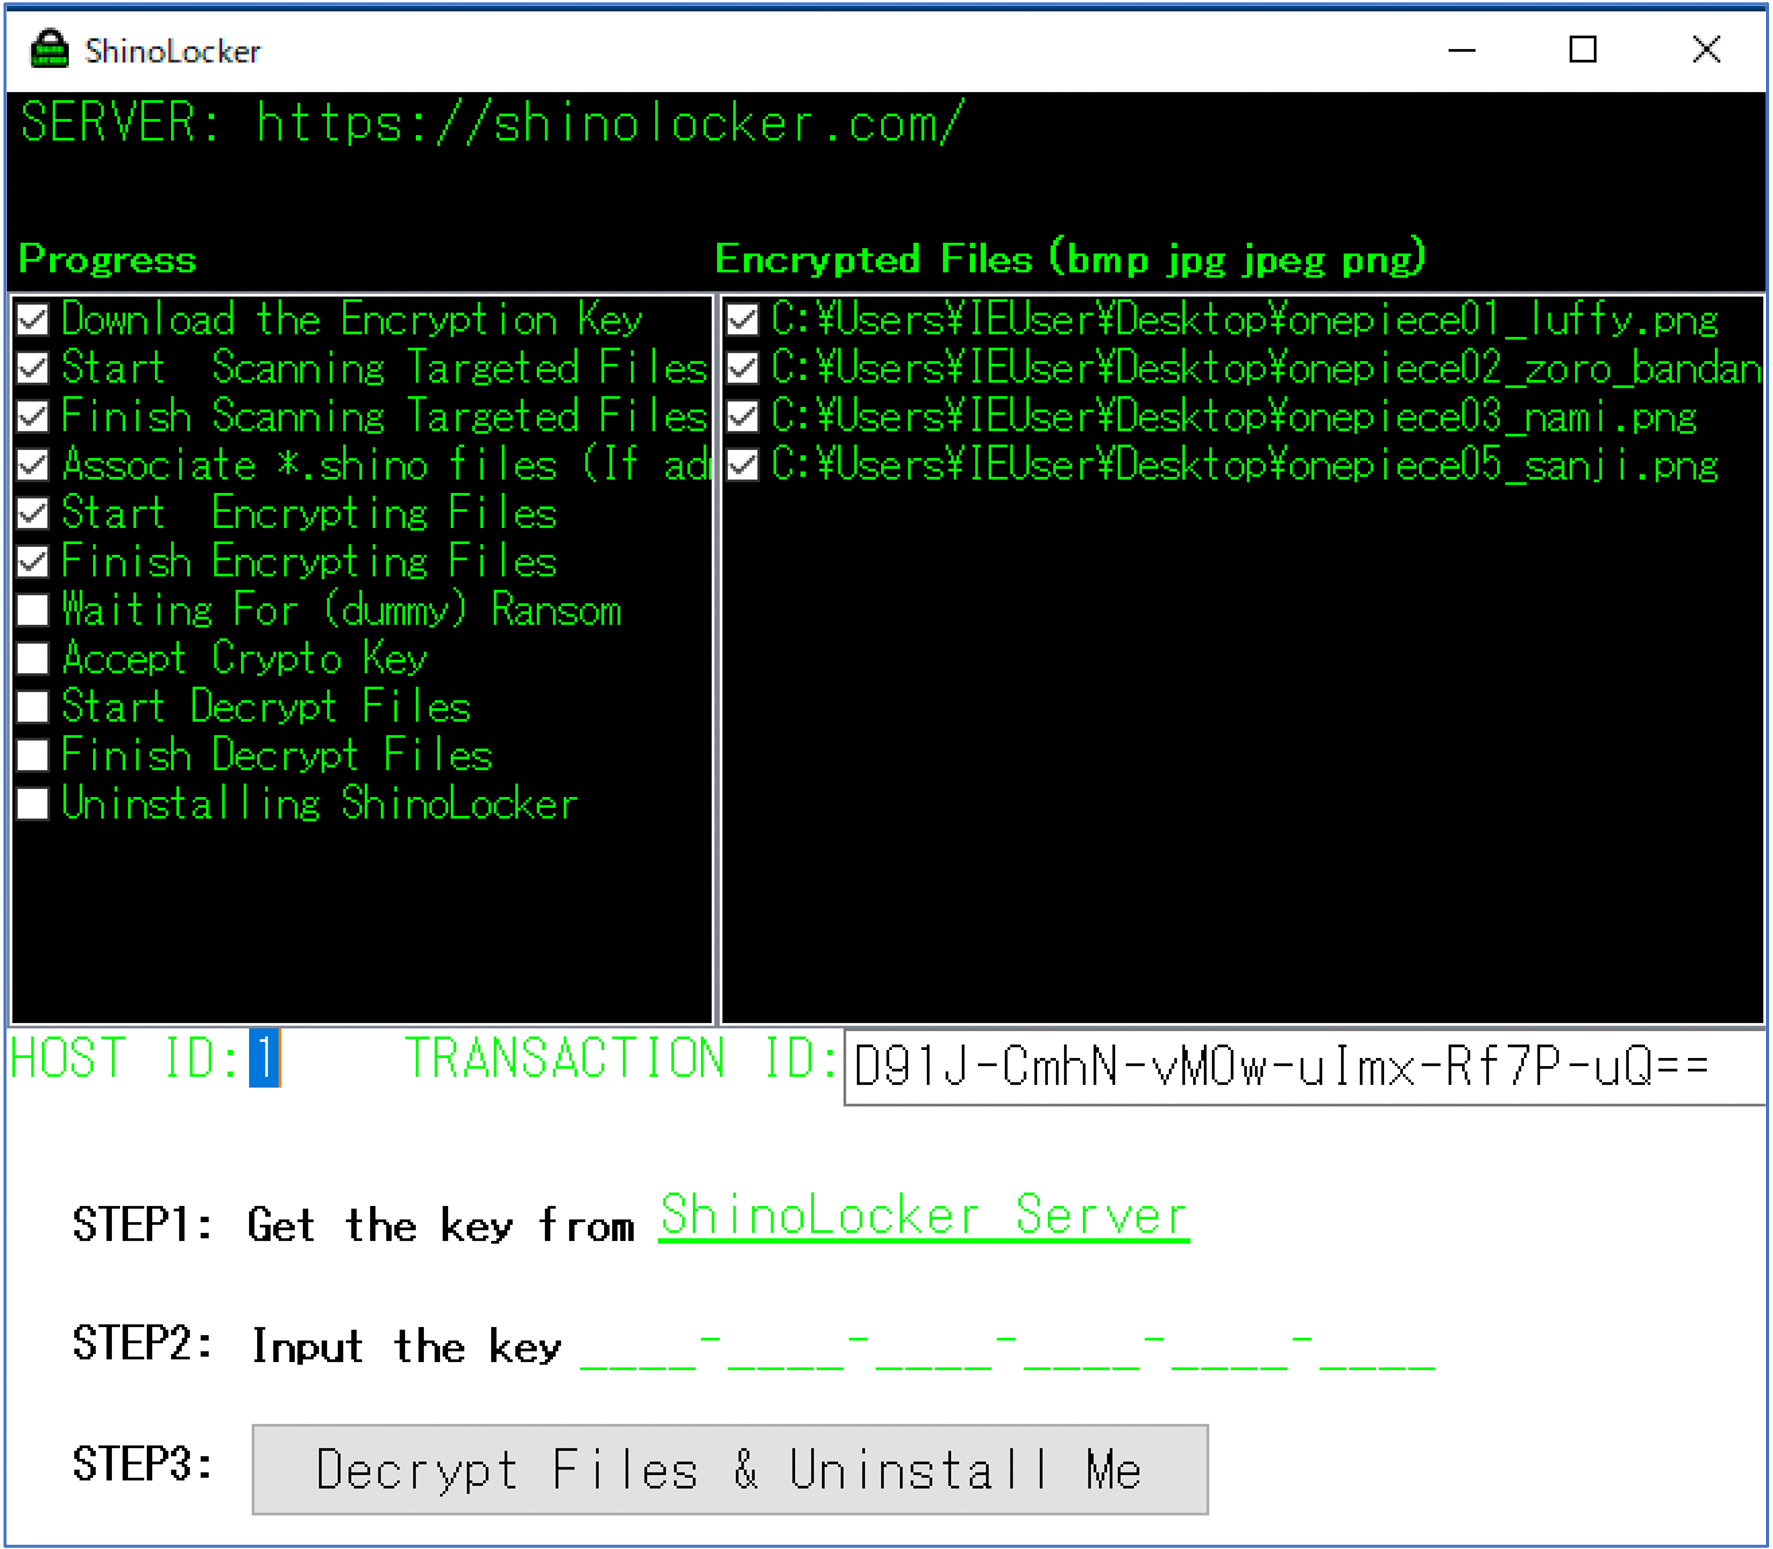
\includegraphics[keepaspectratio,scale=0.45]{pic5.png}
    \end{center}
    \caption{暗号化ファイルを起動後の動作2}
  \end{minipage}
\end{figure}

\section{解析結果}

\subsection{プロセスの親子関係}

採取したログの親子関係を確認したところ、「vssadmin.exe」と「EDuRCHEG.exe」
の二つが呼び出されていることが確認できた。「vssadmin.exe」はボリュームの
シャドウを削除しており、暗号化後のバックアップを困難にするのが目的だと考え
られる。ここでボリュームのシャドウとはマイクロソフトが提供しているサービスの
一種である。(図6)


\begin{quote}
  \begin{math}
    VSS(ボリュームシャドウコピーサービス)とは、Windowsのストレージ管理機能の一つで、指定されたボリューム
    の内容を自動的に複製し、専用の領域に保管する機能。特定の時点における
    ファイルの複製を自動的に作成し、専用の記憶領域で管理する。^{(1)}
  \end{math}
\end{quote}

シャドウの削除を行ってはいるが、windowsに標準で搭載されている機能の一つで
あるので、今回の解析の対象外とした。

\begin{figure}[H]
  \centering
  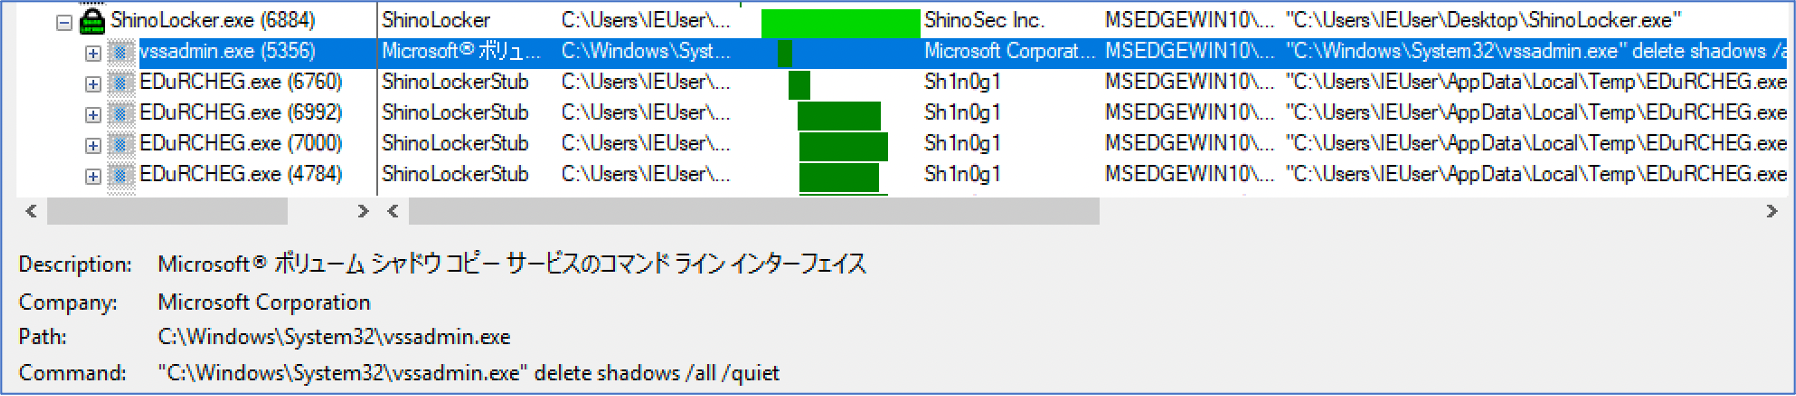
\includegraphics[scale=0.4]{pic7.png}
  \caption{プロセスの親子関係}
\end{figure}

ここで、呼び出されている「EDuRCHEG.exe」は元々コンピュータ内に存在した
ファイルではないので、採取したログを確認したところ、「9K2evkg.exe(EDuRCHEG.exe)」
と「4nMZOU5B.exe(I9BbnQr9.exe)」の二つのファイルが親プロセスShinoLockerによって
生成されていることが確認できた。それらのプロセスと関係を図7,8,9に示す。

\begin{figure}[H]
  \centering
  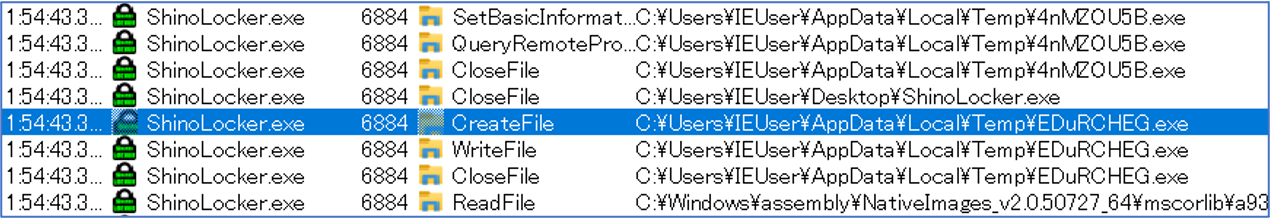
\includegraphics[scale=0.6]{pic8.png}
  \caption{EDuRCHEG.exeの生成プロセスログ}
\end{figure}

\begin{figure}[H]
  \centering
  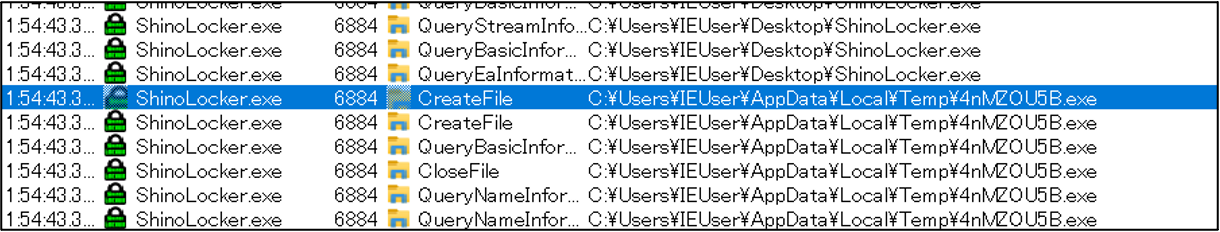
\includegraphics[scale=0.6]{pic9.png}
  \caption{4nMZOU5B.exeの生成プロセスログ}
\end{figure}

\begin{figure}[H]
  \centering
  \fbox{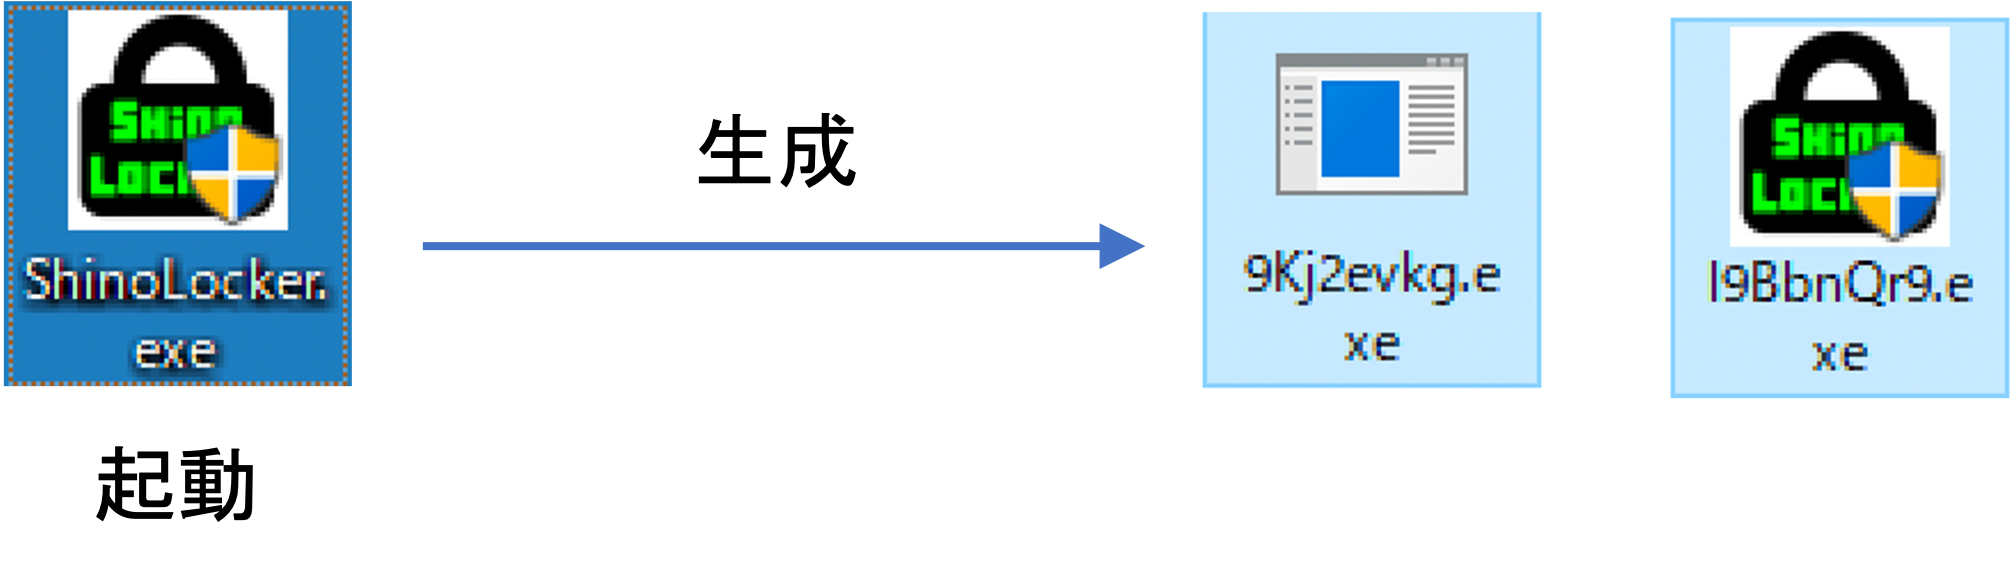
\includegraphics[scale=0.6]{pic15.png}}
  \caption{親子関係図}
\end{figure}

\subsection{9K2evkg.exe(EDuRCHEG.exe)が行っていることの特定}

呼び出されていたこプロセスの内容を確認したところ、\\
\begin{math}
  “C:\backslash Users\backslash IEUser\backslash AppData\backslash Local\backslash Temp\backslash EDuRCHEG.exe” E Wez03hsEhpTFfcIBCH1CnQ
== D91JCmhNvM0wuImxRf7PuQ== “暗号化されたファイルのパス”
\end{math}
\\というログが暗号化されたファイルの数分確認することができた(図10)

\begin{figure}[H]
  \centering
  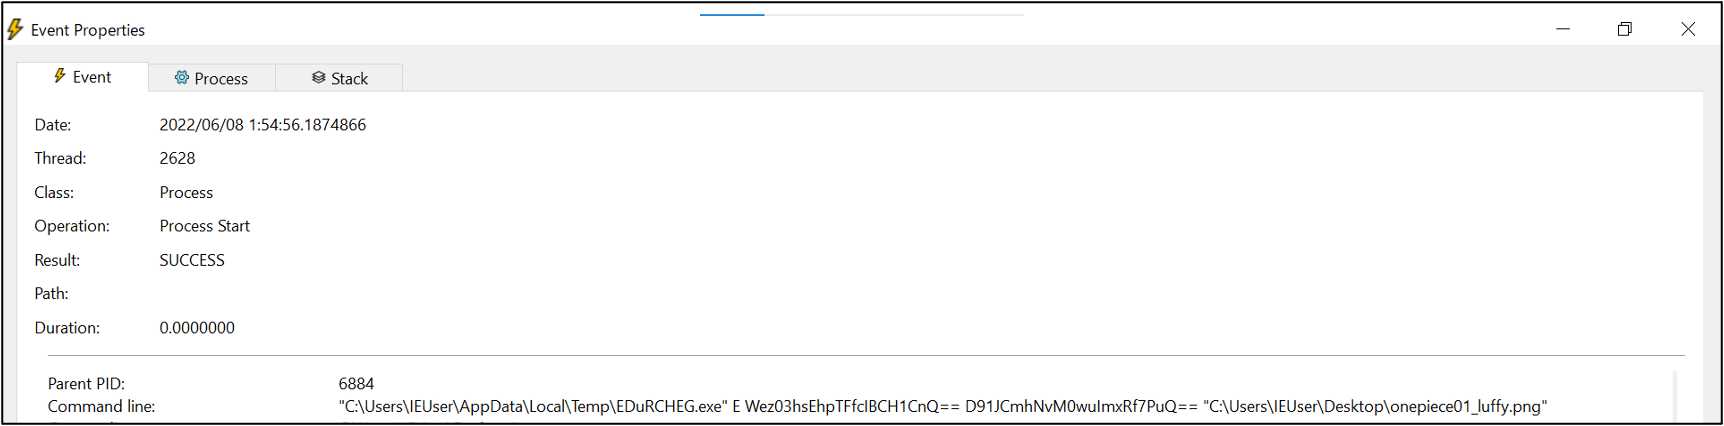
\includegraphics[scale=0.4]{pic10.png}
  \caption{怪しいと思われるプロセス}
\end{figure}

そこで、採取されたログの同様のコマンドをコマンドプロントから呼び出してみたところ、
指定したファイルを暗号化することができた。このとこから、9K2evkg.exe(EDuRCHEG.exe)は
暗号化を行う実行ファイルだと特定することができた。一連の様子を図11,12,13に示す。

\begin{figure}[H]
  \centering
  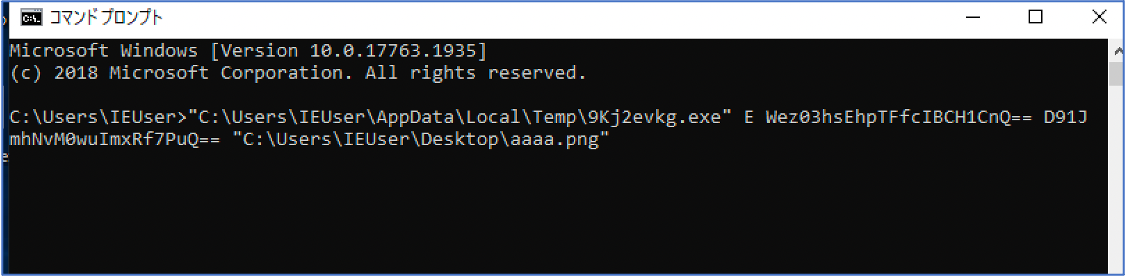
\includegraphics[scale=0.6]{pic11.png}
  \caption{コマンドプロンプトからaaa.pngを暗号化する様子}
\end{figure}

\begin{figure}[h]
  \centering
  \begin{minipage}[b]{0.45\linewidth}
  \begin{center}
    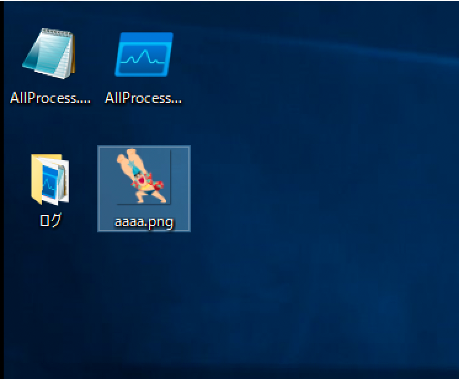
\includegraphics[keepaspectratio,scale=0.7]{pic12.png}
    \end{center}
    \caption{aaa.png暗号化前}
  \end{minipage}
  \begin{minipage}[b]{0.45\linewidth}
  \begin{center}
    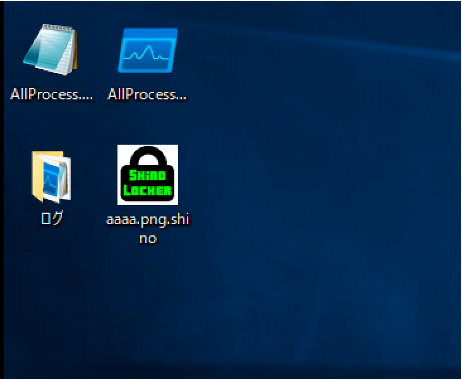
\includegraphics[keepaspectratio,scale=0.7]{pic13.png}
    \end{center}
    \caption{aaa.png暗号化後}
  \end{minipage}
\end{figure}

\subsection{書き込まれたレジストリの解析}
採取したログのうち、「RegSetValue」というレジストリへ書き込みを行う
ログを40個確認することができた(図14)

\begin{figure}[H]
  \centering
  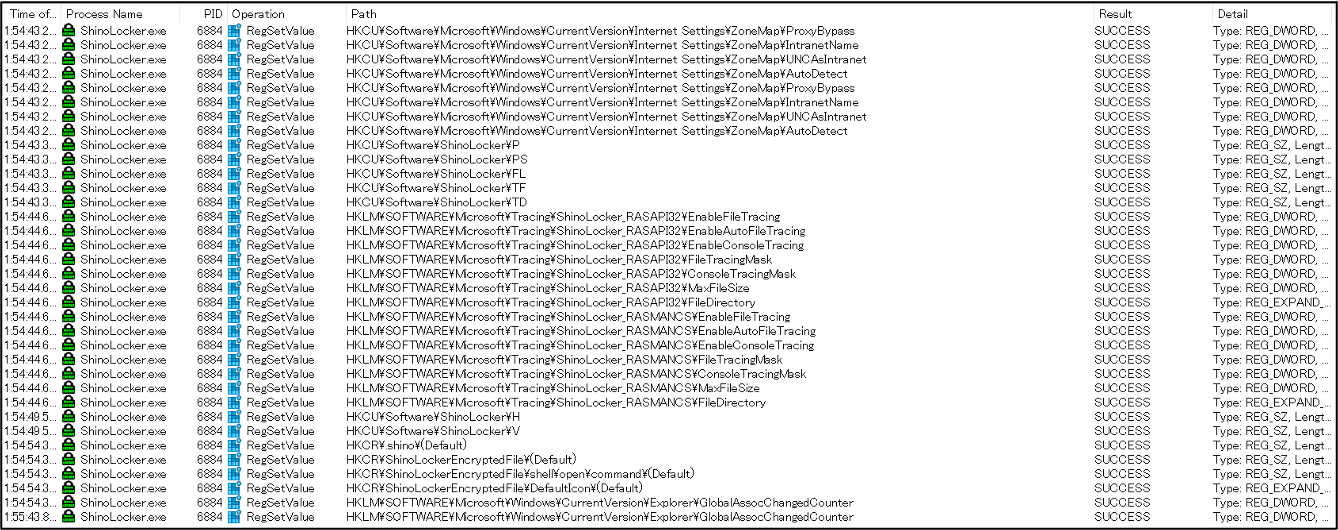
\includegraphics[scale=0.6]{pic14.png}
  \caption{RegSetValueのログ}
\end{figure}

その中で、「.shino」という拡張子の情報を書き込んでいるログを発見することができ、
内容を確認んすると、生成した実行ファイル「4nMZOU5B.exe(I9BbnQr9.exe)」への
関連付けを行っていることが判明した。関連ずけの内容は「.shino」の拡張子の情報を「ShinoLockerEncryptedFile」
に格納するという物であり、「ShinoLockerEncryptedFile」を確認すると、「DefaultIcon」と「shell¥open¥command」
によって、「.shino」の拡張子に対しての起動コマンドとアイコンの設定が施されていた。

\begin{figure}[H]
  \centering
  \begin{minipage}[b]{0.45\linewidth}
  \begin{center}
    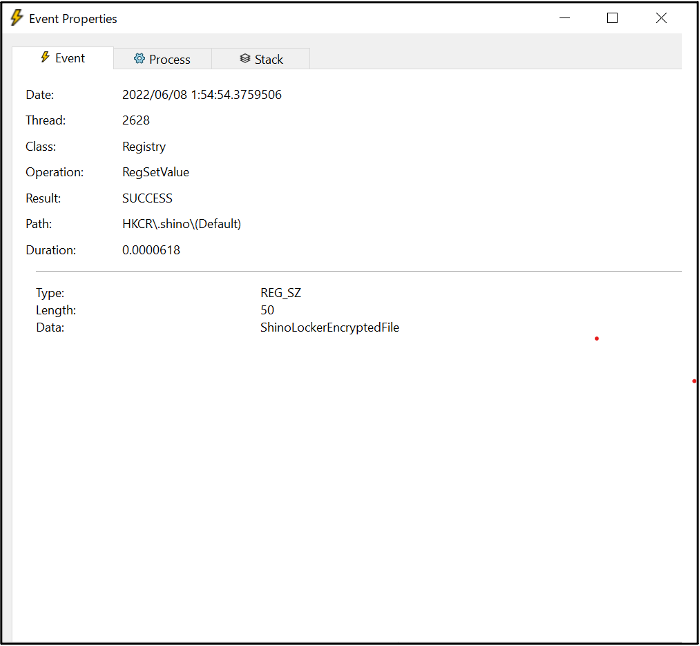
\includegraphics[keepaspectratio,scale=0.45]{pic16.png}
    \end{center}
    \caption{拡張子情報の書き込みログ}
  \end{minipage}
  \begin{minipage}[b]{0.45\linewidth}
  \begin{center}
    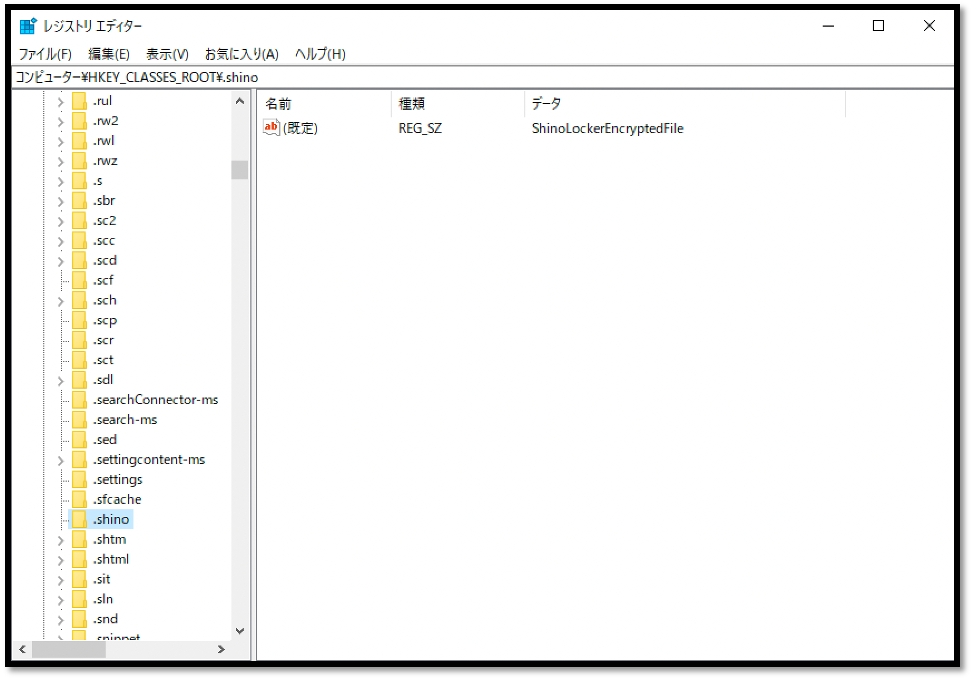
\includegraphics[keepaspectratio,scale=0.36]{pic17.png}
    \end{center}
    \caption{レジストリエディタに.shinoの情報が書き込まれている}
  \end{minipage}
\end{figure}

\begin{figure}[H]
  \centering
  \begin{minipage}[b]{0.45\linewidth}
  \begin{center}
    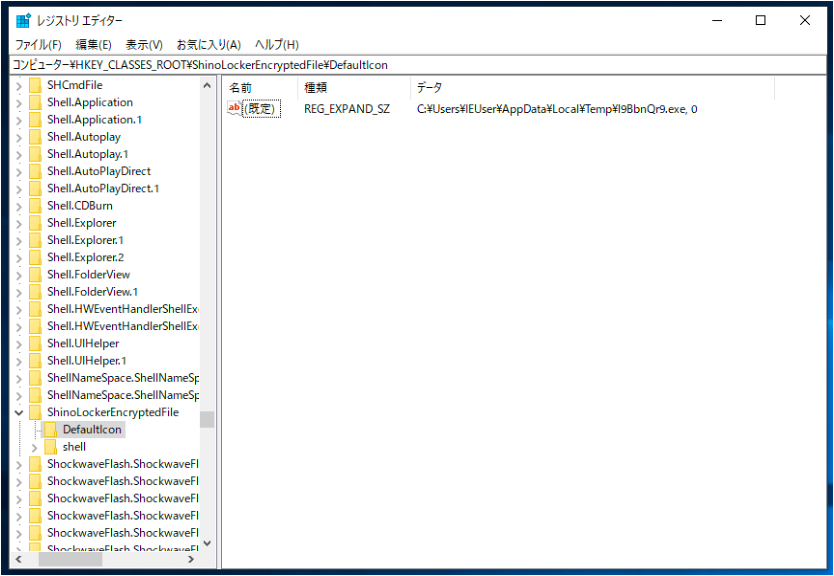
\includegraphics[keepaspectratio,scale=0.4]{pic18.png}
    \end{center}
    \caption{アイコンの設定}
  \end{minipage}
  \begin{minipage}[b]{0.45\linewidth}
  \begin{center}
    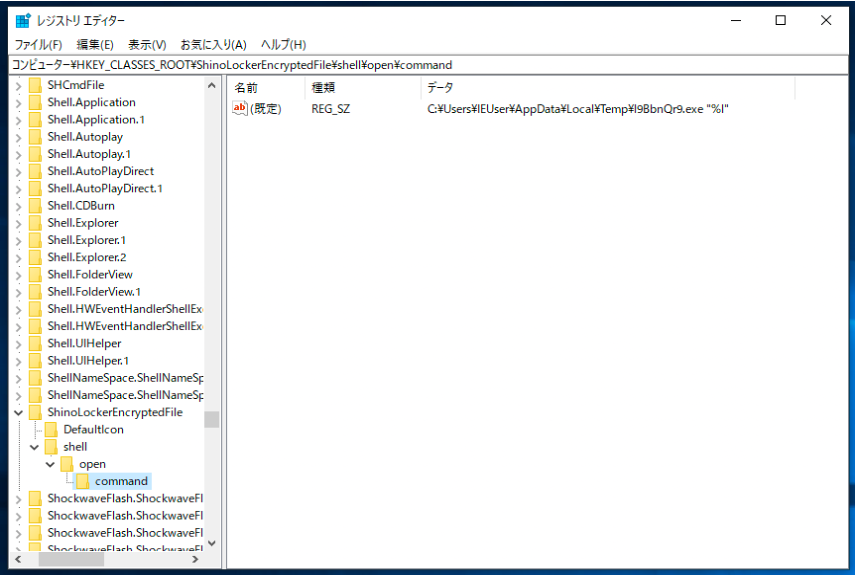
\includegraphics[keepaspectratio,scale=0.4]{pic19.png}
    \end{center}
    \caption{起動コマンドの設定}
  \end{minipage}
\end{figure}

関連付けを行うことで、特定の拡張子に対して実行ファイルを指定することができ、
また、アイコンも指定の物に変更することができる。実行ファイルを指定する原理に
ついて図にまとめる。(2)

\begin{figure}[H]
  \centering
  \fbox{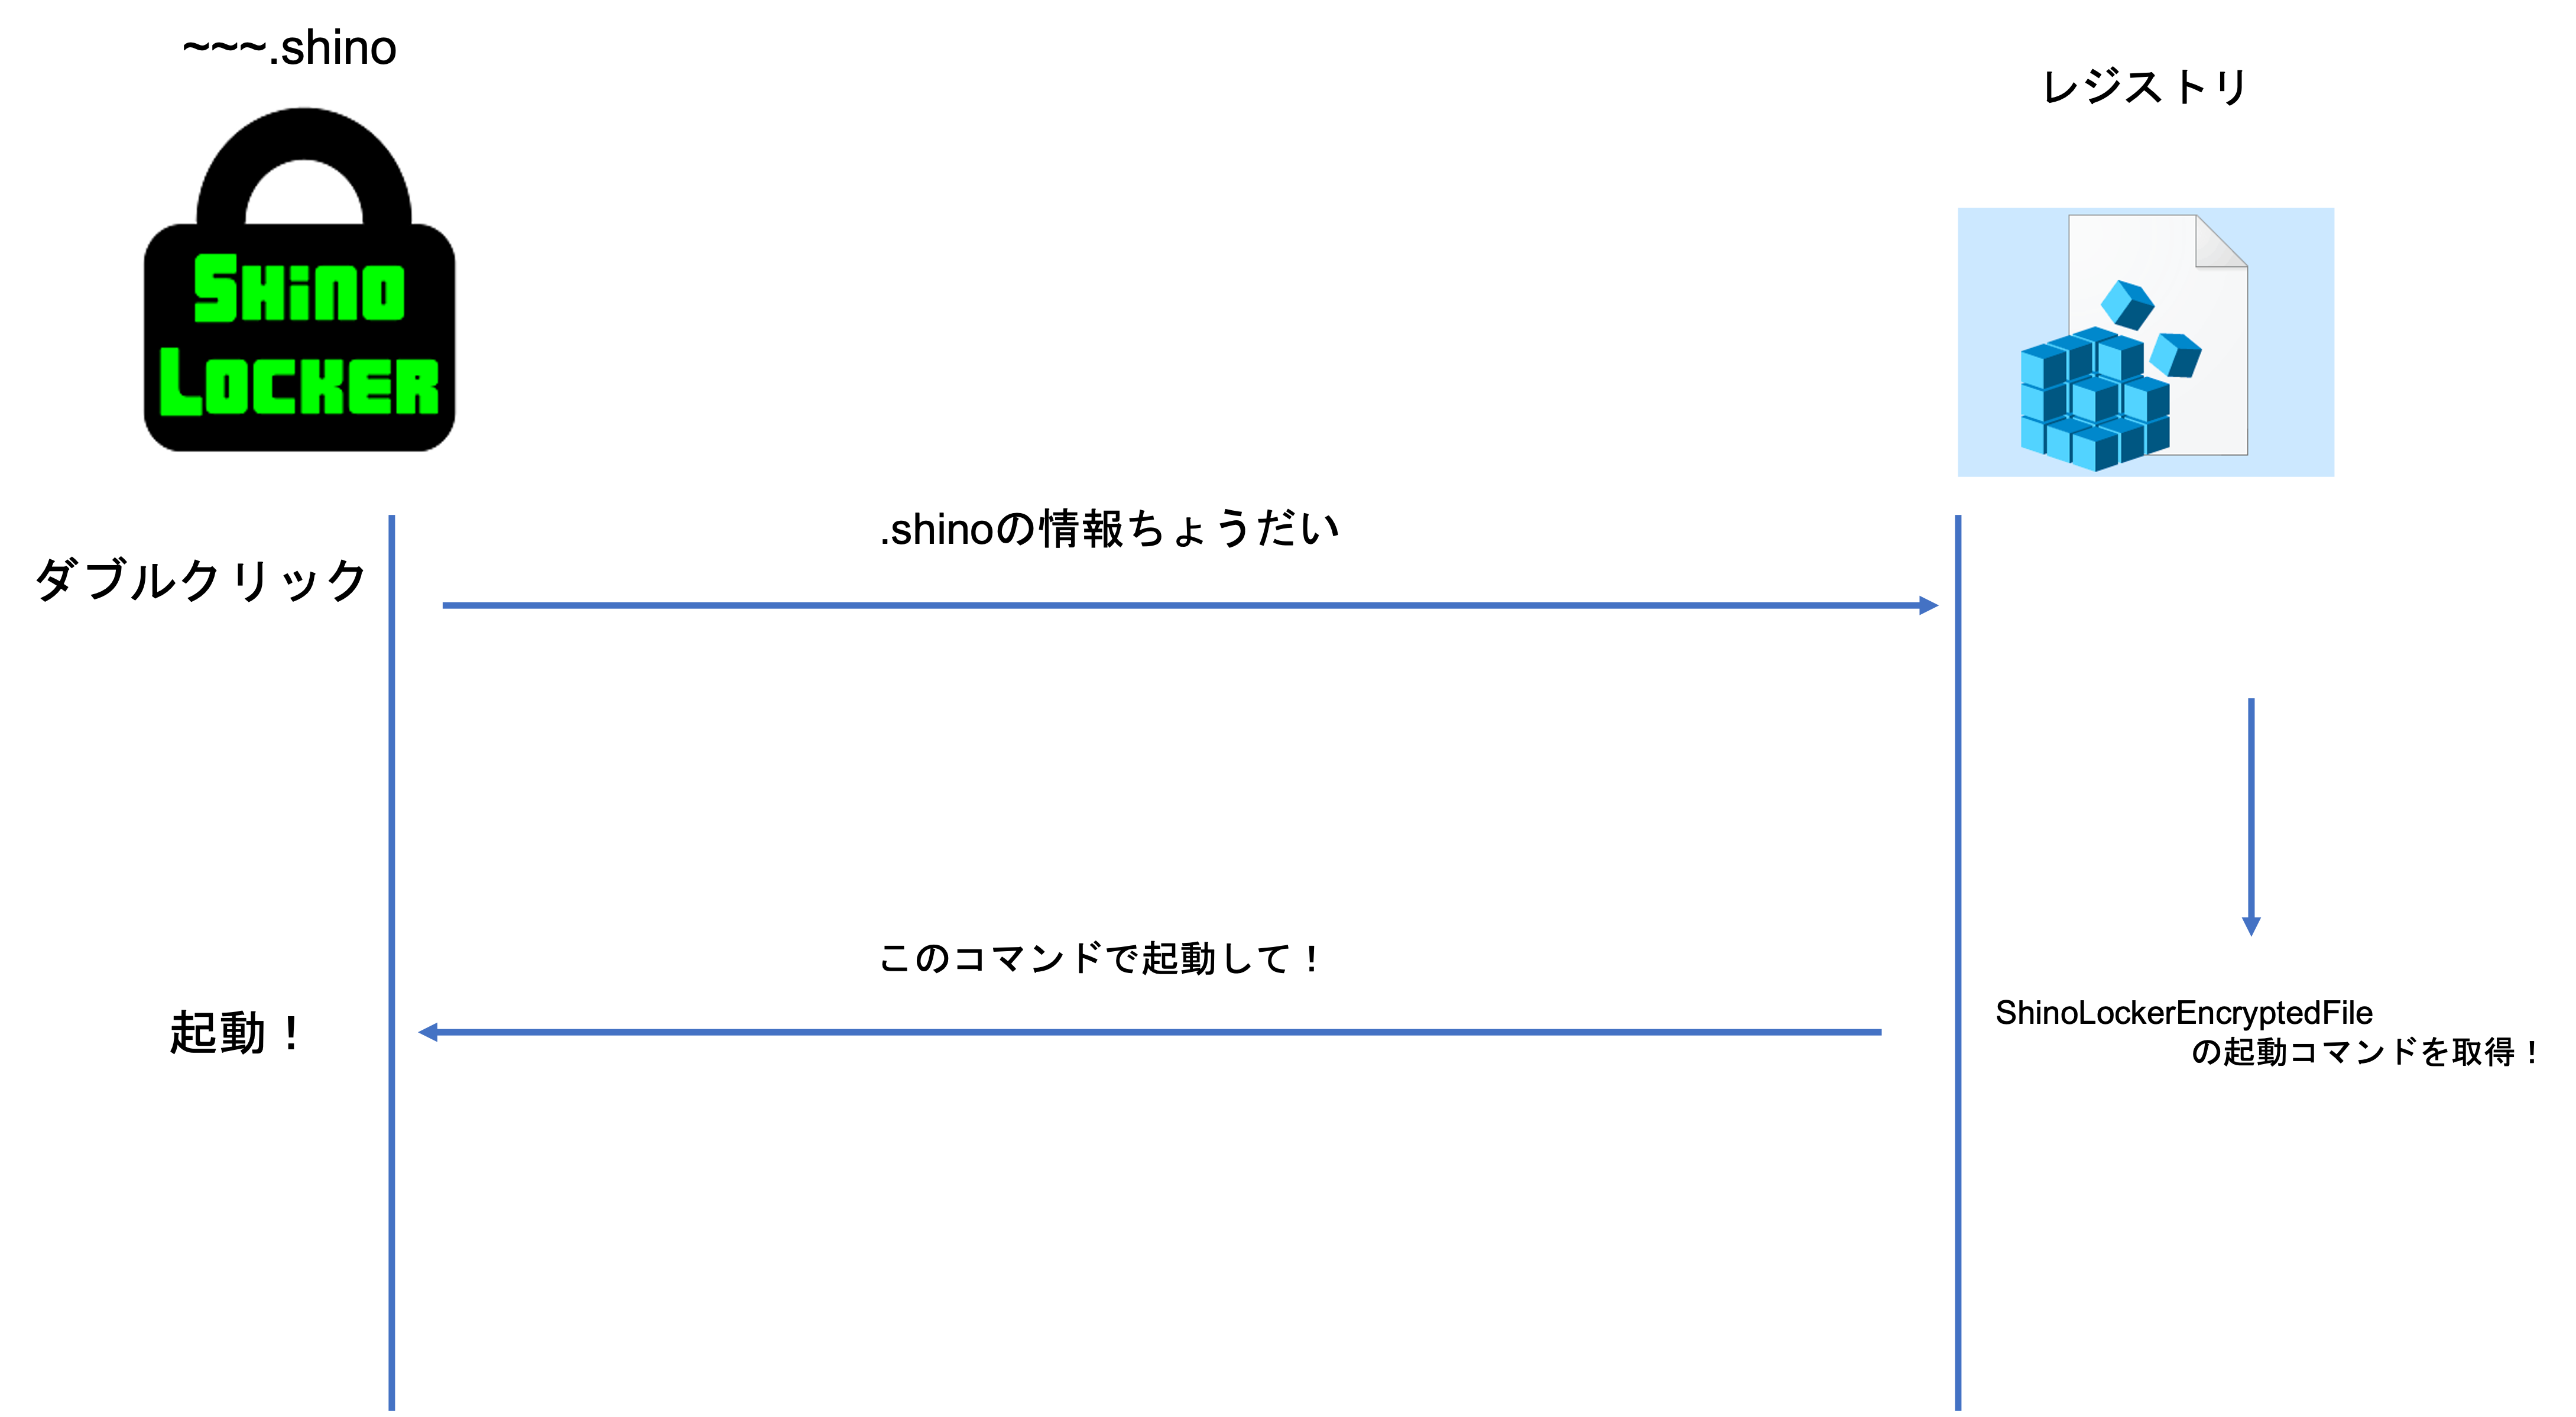
\includegraphics[scale=0.3]{pic21.png}}
  \caption{拡張子とレジストリの関係}
\end{figure}

\subsection{ShinoLockerの一連の動作について}

解析結果から分かったShinoLockerの動作についてまとめる。まずShinoLocker
本体は暗号化を行っておらず、関連付け、実行ファイルの生成など、暗号化やその後の
準備を行う「ドロッパー」として動作していることが分かった。ShinoLockerと生成された
実行ファイルの役割を以下の表2,図20にまとめる。

\begin{table}[h]
  \caption{役割まとめ表}
  \begin{tabular}{|c|c|}
  \hline
  ファイル名                      & 役割                                                                  \\ \hline
  Shino Locker               & 9K2evkg.exe,4nMZOU5B.exeの生成、関連付け情報の書き込み \\ \hline
  9K2evkg.exe(EDuRCHEG.exe)  & ファイルの暗号化                                                            \\ \hline
  4nMZOU5B.exe(I9BbnQr9.exe) & 関連付けの対象、アイコン変更                                                      \\ \hline
  \end{tabular}
  \end{table}
  
  \begin{figure}[H]
    \centering
    \fbox{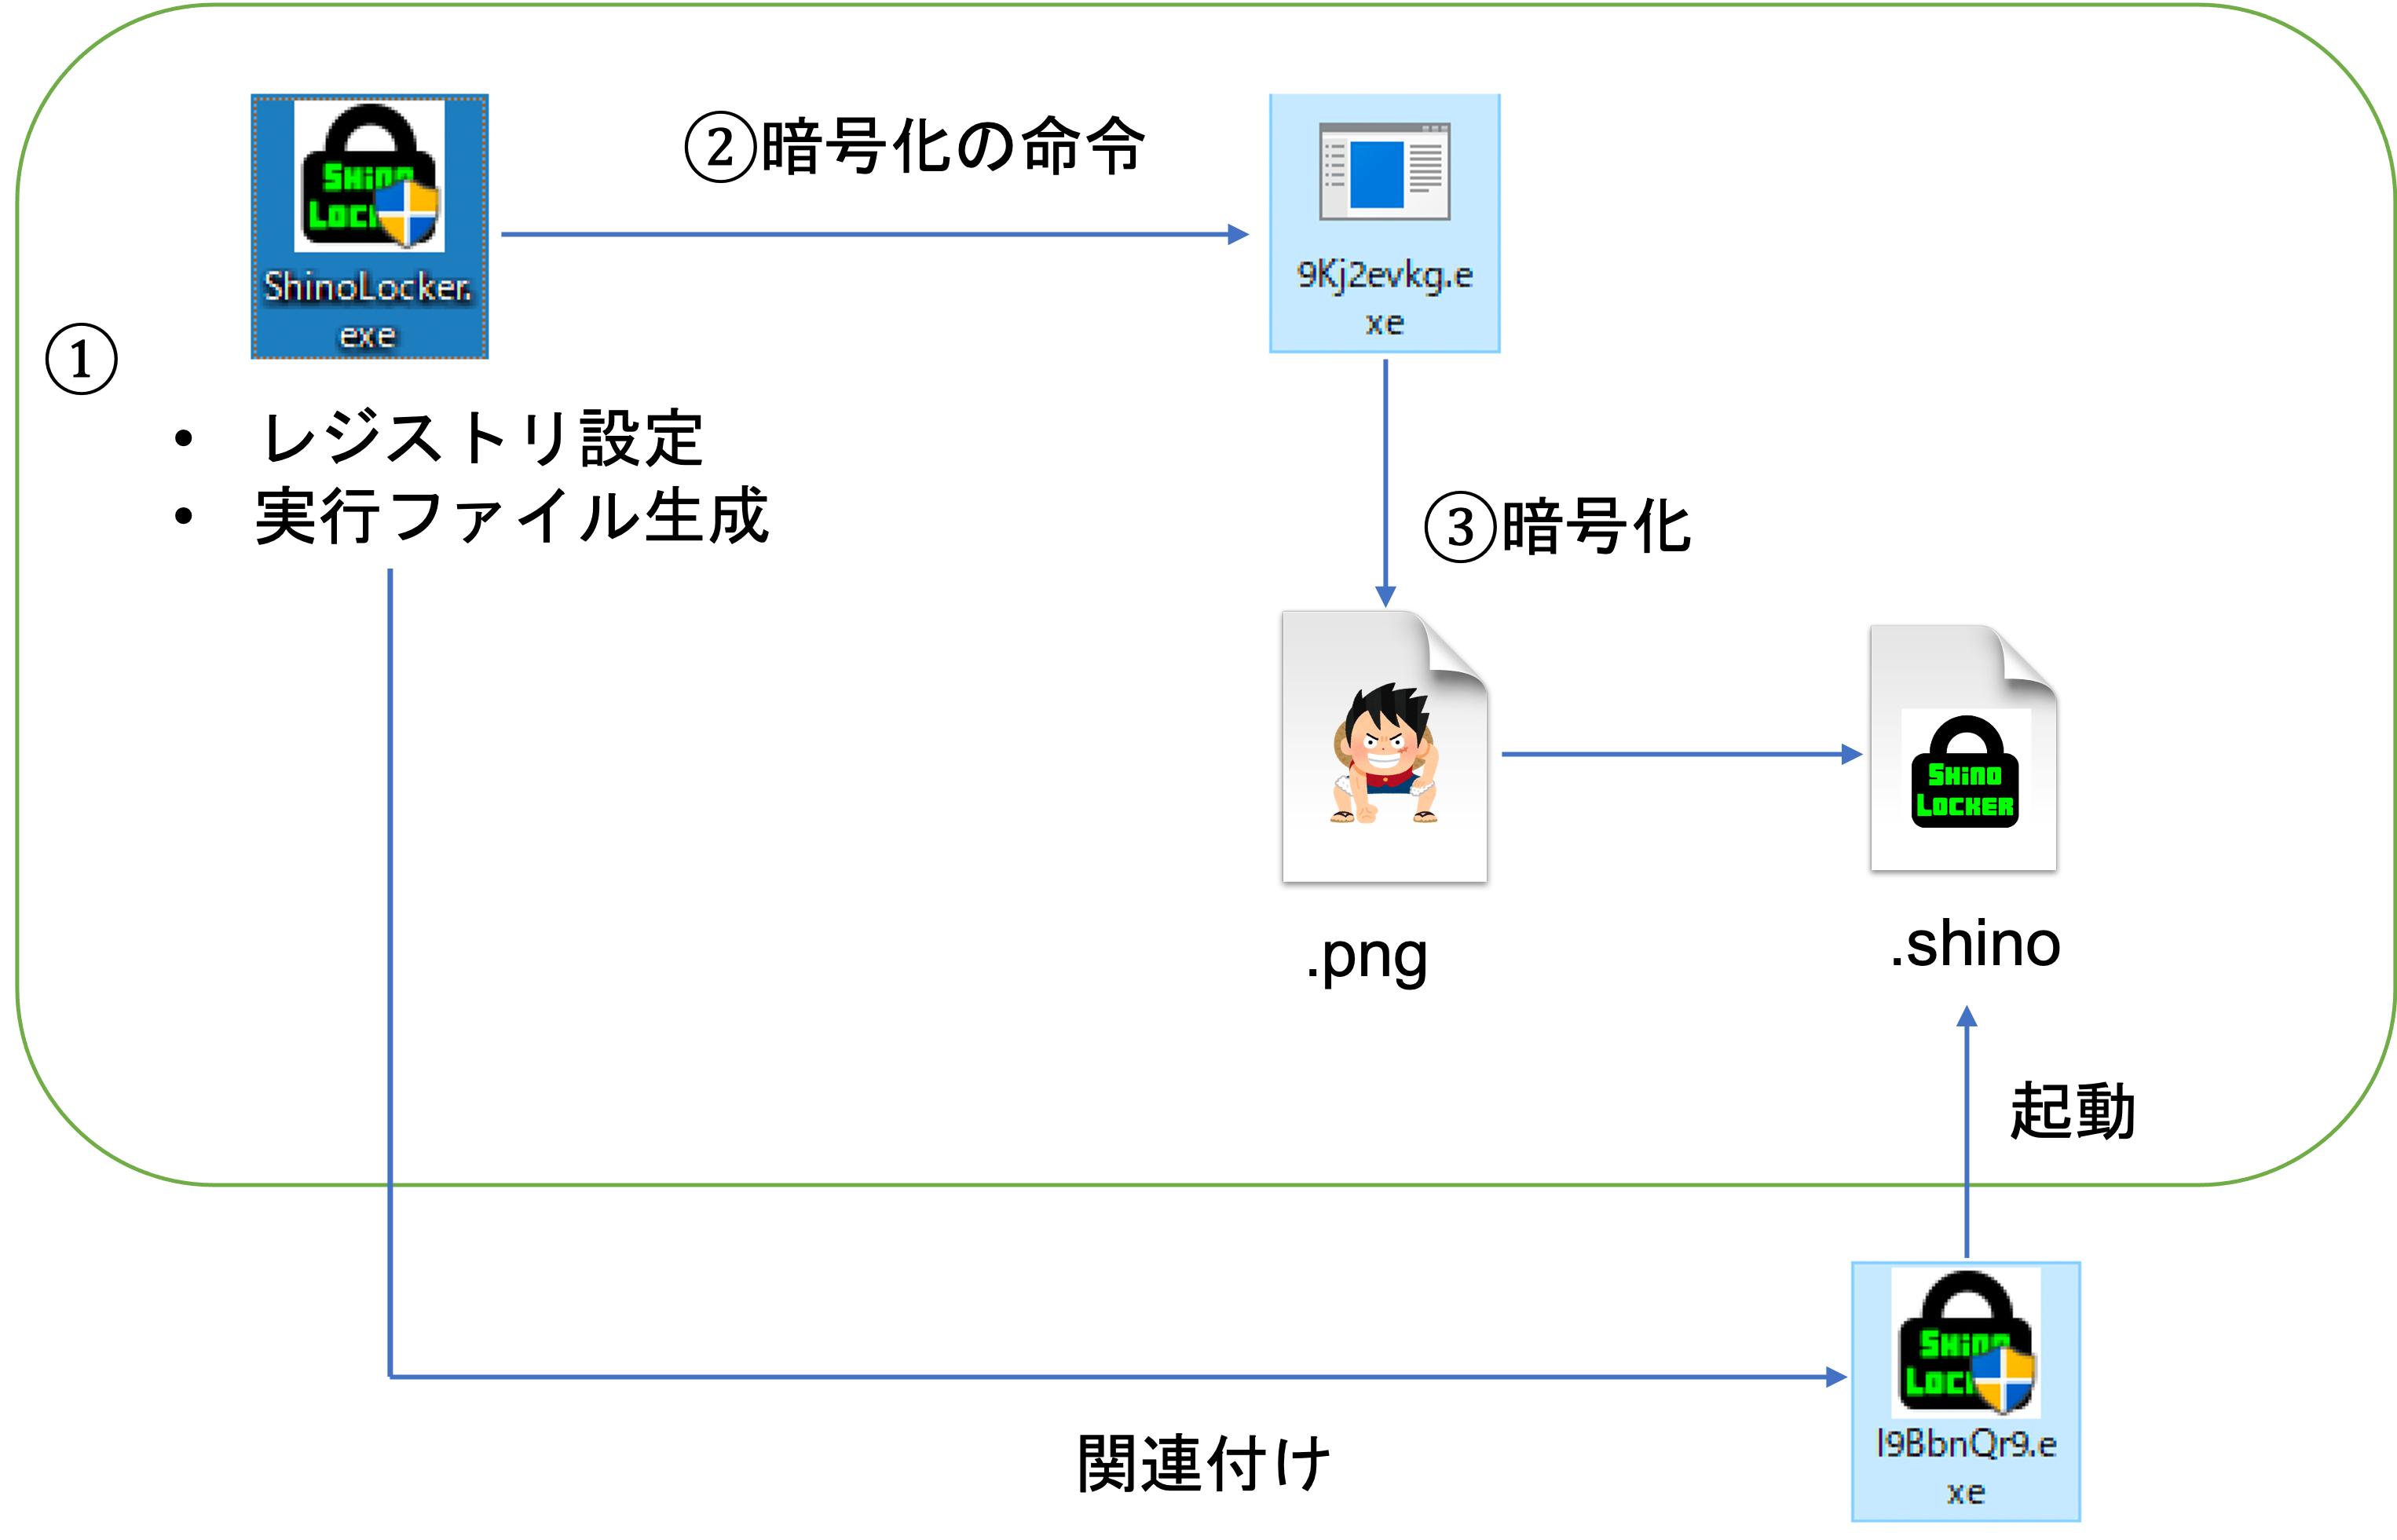
\includegraphics[scale=0.5]{pic20.png}}
    \caption{関係図}
  \end{figure}


\section{今後の課題}
本実験では、ランサムウェアShinoLockerと、それによって生成された実行ファイルの役割を明らかにし、暗号化がどのような手順で行われているのかを
つかむことができた。これにより、暗号化を行う上で、ほとんどのランサムウェアは、はじめに暗号化のための環境を整えることが考えられる。今後は、暗号化を未然に防ぐために
、この暗号化の準備を行うドロッパーが機能した時点で、プログラムがランサムウェアであることを判断し、停止することを目的に、レジストリの情報も含め、さらに詳しい解析を行いたい。
\section{参考文献}

(1) VSS【ボリュームシャドウサービス】 , IT用語辞典 e-Words  \\
\qquad\quad \url{https://e-words.jp/w/VSS.html}

(2) ファイルをダブルクリックしてからアプリが起動するまで \\
\qquad\quad \url{https://tunemicky.blogspot.com/2011/11/blog-post.html}

(3) 令和3年におけるサイバー空間をめぐる脅威の情勢等について 警察庁\\
\qquad\quad \url{https://www.npa.go.jp/publications/statistics/cybersecurity/data/R03_cyber_jousei.pdf}

\end{document}

